\documentclass[a4paper, 12pt]{article}
\usepackage{titling}
\usepackage[margin=3.0cm]{geometry}
\usepackage{graphicx}
\usepackage{amsmath}
\usepackage{amssymb}
\usepackage{lipsum}
\usepackage{hyperref}
\usepackage[style=ieee, url=false, doi=false, isbn=false]{biblatex}
\addbibresource{bibliography.bib}

\begin{document}

\title{\bf Feature and Lazy Learning and the Jamming Transition in Artificial Neural Networks}
\author{
    Hudson Cooper\\ % REDACT FOR SUBMISSION
    King's College London\\
    M.Sc.\ in Complex Systems Modelling
}
\date{\today}

\begin{titlingpage}
\maketitle
\begin{abstract}
\lipsum[1]
\end{abstract}
\end{titlingpage}

\section{Introduction}
Despite the remarkable success of neural networks in a variety of contexts such as vision, speech, natural language processing, drug discovery, and genomics \cite{lecunDeepLearning2015}, there is no cohesive theoretical explanation for this success; the understanding and design of these networks has been almost exclusively guided by empirical work. \\

Why are neural networks able to fit to and generalize from data so well? What criteria and design choices enable these abilities? These crucial questions remain open. Recent advances toward answering them have assumed that a specific regime known as ``lazy learning" provides an adequate description of the behavior of neural networks in practical settings. This paper explores some critical limits to that assumption, mainly by comparing qualitative differences between ``lazy learning" and ``feature learning," a more complex and poorly understood regime that appears to be behind the successes of certain neural architectures, such as convolutional neural networks. 

\section{Background}

\subsection{Double Descent: ``Classical" vs. ``Modern" Regimes}

The success of modern neural networks is in stark contrast to a cornerstone of classical statistical learning: the so-called ``bias-variance trade-off." The bias-variance trade-off holds that more expressive models are more likely to find spurious patterns in data and generalize poorly to new samples, a behavior referred to as ``over-fitting." The trade-off implies that practitioners should seek to find the sweet-spot by building models that are ``as simple as possible, but no simpler." Neural networks, however, typically operate in a highly over-parameterized regime, containing many more parameters than there are data. Neural networks have been shown to be so highly expressive that they are able to interpolate and perfectly classify training data, even when labels have been replaced with pure noise \cite{zhangUnderstandingDeepLearning2017}. Classical statistical learning suggests that neural networks should therefore be extremely prone to over-fitting, but despite their complexity and expressiveness, they are able to generalize extremely well in practical settings.\\

Recent work \cite{belkinReconcilingModernMachine2019} has characterised this phenomena in terms of the so-called ``double-descent" curve, visually represented in figure \ref{doubledescent}. Two distinct regimes of model complexity are separated by the interpolation threshold, the point beyond which models are able to obtain perfect performance on training data. To the left of this threshold is the ``classical" or ``under-parameterized" regime, in which the bias-variance trade-off holds and generalization error follows a U-shaped curve, decreasing to a minimum before increasing to a peak at the interpolation threshold. Past this threshold, however, is the ``modern," ``interpolating," or ``over-parameterized" regime, in which the generalization error again decreases, with the global optimum being found deep in the over-parameterized regime, sometimes in the limit of infinite complexity. This double-descent phenomenology is far from unique to neural networks and has been observed in a variety of other model classes that are expressive enough to perfectly interpolate training data, including random forests, random feature models, and kernel machines \cite{ belkinReconcilingModernMachine2019, belkinUnderstandDeepLearning2018}. Several open questions remain about this modern regime: What are the sufficient conditions for training data to be well fitted and for interpolation to begin? What causes generalization to improve beyond this threshold?

\begin{figure}[ht]
\centering
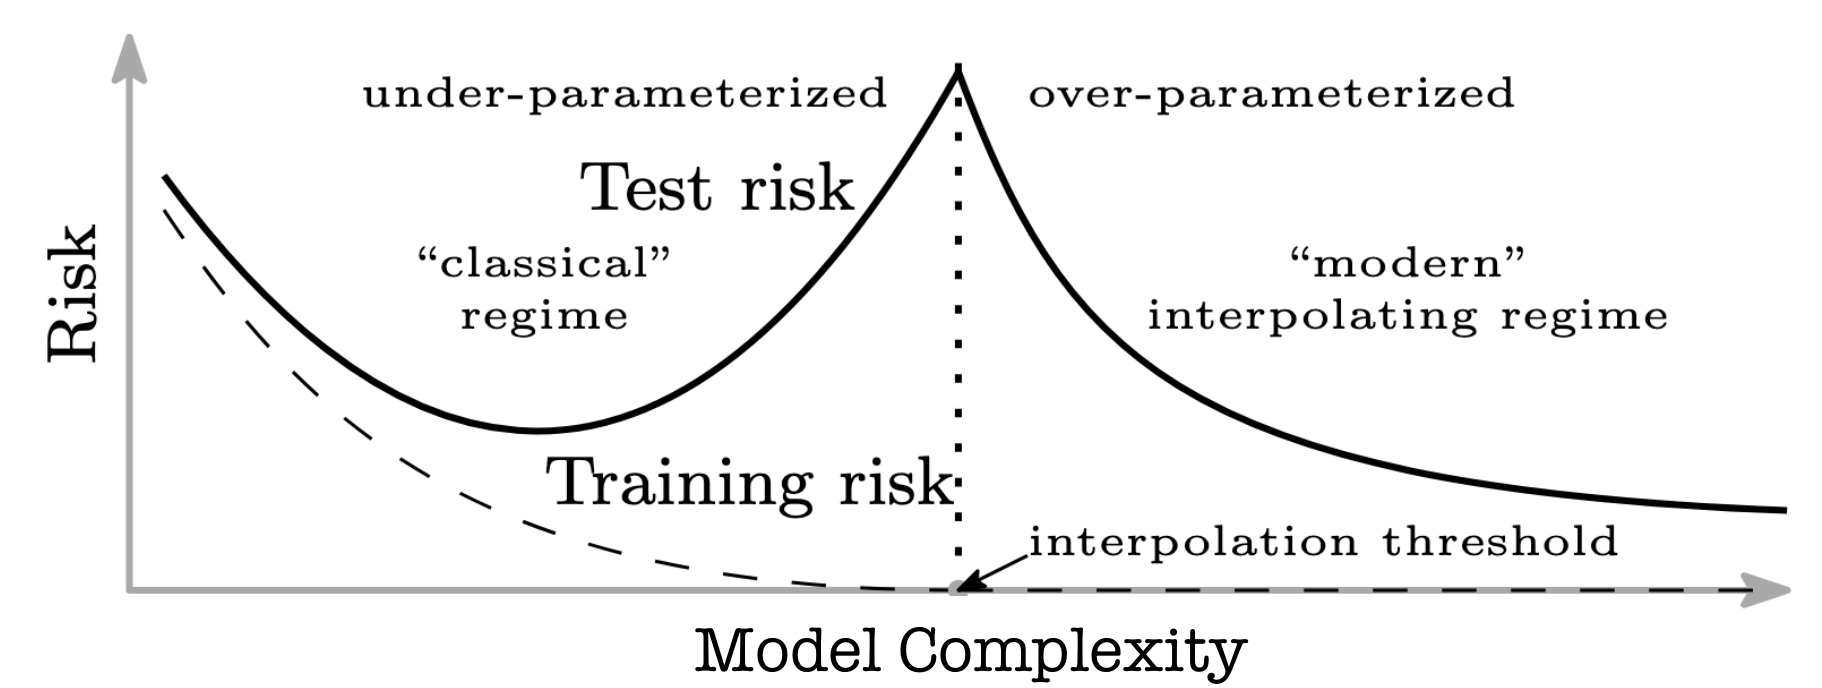
\includegraphics[width=0.7\textwidth]{docs/assets/double_descent_reconciling.png}
\caption{Visual depiction of the double descent curve, adapted from \cite{belkinReconcilingModernMachine2019}. The ``classical" U-shaped bias-variance trade-off is seen in the under-parameterized regime to the left of the interpolation threshold, and a second descent is seen in the over-parameterized regime to the right. Training error (``risk'') is represented with a dashed line, and test error is represented with a solid line.}
\label{doubledescent}
\end{figure}



\subsection{The Jamming Transition}

It is no surprise that highly expressive models, such as over-parameterized neural networks, have global optima associated with arbitrarily small training loss; however, it is highly non-trivial that they are able to attain this vanishing loss without getting stuck in local minima, due to their loss landscapes being generally non-convex or non-smooth in the case of ReLU activations. There are strong similarities between neural networks and statistical-physics models of systems with many interacting components, in particular mean-field glassy systems, which take an exponentially long time (in the number of parameters) to relax to global minima due to extremely rough loss landscapes with many local minima \cite{choromanskaLossSurfacesMultilayer}. These similarities suggest that networks trained with stochastic gradient descent (SGD) from random initialization should converge to high and wide minima despite the existence of deeper local and global minima. In practice, however, SGD almost never encounters any such obstacles, and global minima are easily found \cite{goodfellowQualitativelyCharacterizingNeural2015}.\\

Studying the training dynamics of neural networks undergoing SGD, \cite{baity-jesiComparingDynamicsDeep2019} found that while under-parameterized networks exhibit the hallmarks of glassy dynamics, over-parameterized networks behave in a qualitatively different manner and have loss landscapes of a different statistical structure. On the basis of this finding, the authors conjectured the existence of a phase transition separating these regimes, sharing similarities to the ``jamming" phase transition by which particles form a disordered solid as their density is increased. A similar jamming transition had previously been found separating easy and hard algorithmic phases in several computational optimization problems, including the perceptron \cite{krzakalaLandscapeAnalysisConstraint2007,zdeborovaPhaseTransitionsColoring2007,franzUniversalitySATUNSATJamming2017}. In \cite{geigerJammingTransitionParadigm2019} and \cite{spiglerJammingTransitionOverparametrization2019}, the authors empirically explore the boundary between the under- and over-parameterized regions of neural networks, finding that their behavior near the interpolation threshold does, in fact, share similarities to jamming, falling in the same universality class as elliptical particles (in contrast to the jamming of spherical particles as is seen in the perceptron). In particular, they found that this transition is sharp and has a discontinuous jump in the number of unsatisfied constraints, i.e. the number of data that are poorly fit, at the boundary. They furthermore argue that the number of unsatisfied constraints as a fraction the number of degrees of freedom is not sufficiently large enough to form local minima in the overparameterized regime, offering a simple explanation as to why such networks do not get stuck.

\subsection{``Lazy Learning" in Over-Parameterized Networks}

By taking the limit as network width goes to infinity, a correspondence between wide neural networks and the so-called ``lazy-learning" regime has been established, resulting in a recent flurry of theoretical progress. In particular, \cite{jacotNeuralTangentKernel2018} showed that gradient-descent on network parameters corresponds to gradient-descent on network outputs with respect to a kernel known as the ``Neural Tangent Kernel" (NTK). In the infinite width limit, the NTK converges to a deterministic limiting kernel that depends only on the network architecture, is independent of parameter initialization, and is constant throughout training. This limit is referred to as the ``lazy learning" limit because the NTK does not depend on the data-set. Although the derivation is exact only in the infinite-width limit, experimental evidence in \cite{jacotNeuralTangentKernel2018} shows good agreement between both the training dynamics and final predictions of the limiting NTK machine and networks trained in the large but finite width setting across a variety of practical architectures. Further work in \cite{allen-zhuConvergenceTheoryDeep2019} proved that the training dynamics of finite but over-parameterized networks rapidly converge to those of the corresponding limiting NTK.\\

In the the lazy learning limit, network outputs can be expressed as a first-order Taylor expansion of the network about its initial weights at any time during training \cite{leeWideNeuralNetworks2019}. For a network $f_\theta$ with initial parameters $\theta_0$ and an initialization such that $f_{\theta_0} \approx 0$\footnote{Alternatively, one can define the network output to be $f_{\theta}(x) - f_{\theta_0}(x)$ as is seen in \cite{chizatLazyTrainingDifferentiable2020}}, we have that
\begin{equation}
    f_\theta(x) \approx \nabla_\theta \left.f_\theta(x)\right|_{\theta=\theta_0} \cdot (\theta - \theta_0)\,.
\end{equation}
In other words, networks in the lazy-learning regime are linear models of random features given by the gradient of the network with respect to its parameters at initialization. The inner product in this random feature space converges to the limiting NTK as the number of parameters goes to infinity, suggesting that finite-width networks can be conceptualized as finite-rank approximations to the limiting kernel machine, connecting finite-width networks to the random features (RF) models studied in \cite{rahimiRandomFeaturesLargeScale2008,meiGeneralizationErrorRandom2019}.

\subsection{Theoretical Victories of Lazy Learning}

The lazy-learning regime offers a greatly simplified point of view from which to understand the training dynamics and convergence properties of overparameterized neural networks. The authors of \cite{allen-zhuConvergenceTheoryDeep2019} offer an explanation of the mechanisms by which over-parameterized neural networks are able to avoid spurious local minima. They show that networks in the lazy regime have ``nearly-convex" loss in a sufficiently large neighborhood around initialization, allowing convergence to the global minimum in polynomial time. This explanation is compatible with the arguments made in the jamming transition literature, i.e. \cite{geigerJammingTransitionParadigm2019,spiglerJammingTransitionOverparametrization2019}, as they both rely on the non-existence of local minima to explain convergence times faster than the exponential times expected in glassy systems.\\

Due to lazy learning's connection to random-features models, it has also opened the door to understanding the generalization capabilities of networks in the overparameterized regime. RF models, as introduced in \cite{rahimiRandomFeaturesLargeScale2008}, are linear functions of pointwise nonlinearities applied to fixed random linear transformations of input data. They can be conceptualized as two-layer neural networks in which the first-layer weights (with width equal to the number of random features) are fixed at their independently random initialized values and the second layer weights are optimized freely. Note that for networks with a single hidden layer, the NTK can be exactly described by this formulation, but deeper networks require the introduction non-independently distributed first-layer weights \cite{chizatLazyTrainingDifferentiable2020}. For regression on random input data with linear or Gaussian-process target functions (classification is similarly examined in \cite{dengModelDoubleDescent2020}), the authors of \cite{meiGeneralizationErrorRandom2019} develop precise asymptotic predictions for the generalization error of a RF model as the number of parameters $N$, the number of data $P$, and the input dimensionality $d$ are sent to infinity with their ratios fixed. Remarkably, they are able to recover the full double-descent phenomenology in this simplified setting, including the features that the test error diverges at the interpolation threshold, as is predicted in \cite{geigerScalingDescriptionGeneralization2019}, and that the global minimum of test error occurs in the infinitely over-parameterized regime, i.e. $N/P\rightarrow\infty$, as is predicted in \cite{belkinReconcilingModernMachine2019,belkinUnderstandDeepLearning2018} for kernel machines.\\

Building on the work of \cite{meiGeneralizationErrorRandom2019} and \cite{ geigerScalingDescriptionGeneralization2019}, which explores the role of initialization variance of the finite-rank NTK on generalization error, \cite{dascoliDoubleTroubleDouble2020} offers a ``modern" treatment of the bias-variance relationship beyond the interpolation threshold. This work disentangles the generalization error in the RF model into its constituent components of bias and multiple sources of variance, including the initialization variance of the random features, sampling variance of the data-set, and additive noise in the target variables. The theoretical predictions made in this simplified RF setting qualitatively match the empirical bias-variance decompositions made in \cite{nealModernTakeBiasVariance2019} for real neural networks, giving credibility to the RF model's ability to explain the behavior of neural networks in the overparameterized regime.

\subsection{Feature Learning}

Despite its success in explaining some of the crucial features of training and generalization in neural networks, the lazy learning perspective misses an important aspect of modern neural networks and deep learning: the role of ``feature learning."  The authors of \cite{chizatLazyTrainingDifferentiable2020} argue that the lazy-learning phenomenon occurs due to an implicitly chosen factor which controls how model parameters scale at initialization against network width. By making this scaling factor explicit, it is possible to force a network to train either in the lazy-learning regime or in the very different ``feature-learning" regime, in which the NTK is no longer constant and evolves throughout training in a manner dependent on the structure of the data. The feature-learning regime is also referred to as the ``mean-field" limit and is explored in some previous works, e.g. \cite{meiMeanFieldView2018}. While the dynamics of lazy learning can be described by a linear ordinary differential equation (ODE) of the network outputs and the constant NTK, the dynamics of feature-learning must be described by a more complex partial differential equation (PDE) which also depends on the empirical distribution of the activations of the hidden neurons. This increased complexity makes the feature-learning regime much harder to study from a theoretical standpoint.\\

 While \cite{allen-zhuConvergenceTheoryDeep2019} guarantees the convergence of lazy-trained networks, it is not immediately obvious that this regime is desirable. In particular, the role of feature learning in the ability of a neural network to generalize to unseen data is still poorly understood. Convolutional neural networks (CNNs) trained in the feature-learning regime have been found to outperform those trained in the lazy-learning regime, suggesting that lazy-learning does not account for the profound success of these networks \cite{chizatLazyTrainingDifferentiable2020}. On the other hand, \cite{geigerDisentanglingFeatureLazy2020} found lazy learning to out-perform feature learning in fully-connected networks (FCNs) with a degree of out-performance that depends on the data-set. This suggests that network architecture and the structure of data play important roles in determining which regime is better. The mechanisms at play, including the role of network depth and other architectural choices on the quality of the learned features and the effects of feature learning on the location of the interpolation threshold, are poorly understood and remain important open questions in modern machine learning. The authors of \cite{geigerDisentanglingFeatureLazy2020} remark that future studies of deep learning should note in which regime their study was conducted, as it is likely that this affects their results.

\section{Methods and Results}
\subsection{The Model}

In order to study the effects of feature-learning on the convergence and generalization capabilities of neural networks, we consider a variation of the random-features model analyzed in \cite{meiGeneralizationErrorRandom2019}. Recall that the random-features model can be described as a two-layer neural network with the first layer weights frozen at their randomly initialized values and the second layer weights freely optimized. We instead train both layers, periodically freezing the first layer and examining the properties of the feature-space spanned by the activations. \\

Consider a scalar-valued two-layer neural network with inputs $x \in \mathbb R^d$, weights $w \in R^{h\times d}$ given by 
$$
    f(x, w, a) = \frac{1}{h}\sum_{i=1}^N a_i \sigma(x^Tw_i) 
$$
where $w_i \in \mathbb R^d$ is the $i^\text{th}$ row of w, $a_i \in \mathbb R$. For randomly initialized $w$, this is the RF model with $N$ degrees of freedom.

\subsection{Feature Learning Near the Generalization Cusp}
\subsection{The Effects of Regularization}

\section{Discussion}

Unclear if the lazy/feature learning regimes are even meaningful in the underparameterized regime.
Unclear whether the network I trained was in lazy or feature learning regimes, and unclear how this may have affected whether the changing first layer actually corresponded to feature learning.

Unclear that using evolving first layer was an appropriate model for feature learning\\
- could instead consider NTK at different times during training, but this is a bit odd because we are no longer taylor expanding around initialization but instead taylor expanding around different points in the training process. However, it's worth exploring how NTK feature space changes over time
- In order to study the gradual effects of the emergence of learned features, ..... (rather than the sharp transition we would have seen if we used values of alpha on either side of the lazy/feature learning transition)

Still poorly understood:\\

- why, when, and how feature learning improves generalization\\
- how the location of the interpolation threshold is affected by feature learning\\
- how the ability of a network to build quality features depends on architecture (and relationship to inductive bias) \\
- the role that feature learning plays in the emergence of the jamming phenomenology\\
- whether the convergence guarantees of lazy learning can be extended to feature learning

\subsection{Conclusion}

Due to the qualitative differences between the jamming transition in the lazy-learning and feature-learning regimes, it is not obvious that the insights into convergence and generalization built in the lazy-learning context can be readily adapted to the feature-learning regime. Identifying these qualitative differences is a step towards building tractable models for describing the properties of networks undergoing feature-learning, which will be crucial to understanding how specific design choices in modern neural architectures have led to state-of-the-art performance and guiding better design choices in the future.

\printbibliography
\end{document}